%+++++++++++++++++++++++++++++++++++++++++++++++++++++++++++++++++++++
%Modelo de TCC da Universidade Tecnológica Federal do Paraná (UTFPR) - Campus Toledo
%Baseado nas orientações do estilo abntex2 (http://linorg.usp.br/CTAN/macros/latex/contrib/abntex2/doc/abntex2.pdf)
%Autor: Felipe Walter Dafico Pfrimer
%Ultima atualização: 04/06/2021
%
% Instruções: 
%	1 - Compile o modelo original;
%	2 - Leia o capítulo 1 do pdf;
%	3 - Acrescente seu texto, procurando organizar os capítulos nas pastas Caps;
%	4 - Se houver, procure organizar os apêndices na pasta Apendices;
%	5 - Se houver, procure organizar os anexos na pasta Anexos;
%	6 - Descomente a linha "\usepackage[a-1b]{pdfx}" para gerar a versão final em PDFA

%+++++++++++++++++++++++++++++++++++++++++++++++++++++++++++++++++++++
%Tipo de documento ABNTEX2:
\documentclass[12pt,openright,oneside,a4paper,
%sumario=tradicional, % para o recomendado pela ABNT utilize sumario=abnt-6027-2012
sumario=abnt-6027-2012,
chapter=TITLE,  % títulos de capítulos convertidos em letras maiúsculas
section=TITLE,  % títulos de seções convertidos em letras maiúsculas
subsection=Title, % títulos de subseções convertidos em letras maiúsculas
subsubsection=Title, % títulos de subsubseções em letras maiúsculas
subsubsubsection=TITLE, % títulos de subsubsubseções em letras maiúsculas
english,french,spanish,brazil]{abntex2}
%Observe que a ABNT NBR 14724:2011 (seção 5.1) recomenda que os documentos sejam impressos no anverso e no verso das folhas. Isso é obtido com a opção twoside.

%+++++++++++++++++++++++++++++++++++++++++++++++++++++++++++++++++++++
%Pacotes para língua portuguesa do Brasil (código recomendado pelo estilo abntex2):
\usepackage{ifxetex}
\ifxetex
    \usepackage{fontspec}
    \defaultfontfeatures{Ligatures={TeX}}
\else
    \usepackage[utf8]{inputenc}
    \usepackage[T1]{fontenc}
\fi

%Observação: Quando um documento é compilado com xelatex, os pacotes inputenc e fontenc não devem ser incluídos ao preâmbulo do documento. Ao invés desses pacotes, geralmente fontspec é usado. O código anterior de preâmbulo torna flexível a compilação do documento, que pode tanto ser realizada da forma tradicional com pdflatex quanto com xelatex, uma vez que inclui seletivamente os pacotes adequados para cada compilador (página 14 do link http://linorg.usp.br/CTAN/macros/latex/contrib/abntex2/doc/abntex2.pdf).

%+++++++++++++++++++++++++++++++++++++++++++++++++++++++++++++++++++++
% Informações do TCC: Editar o arquivo info_tcc.tex com todas as informações do TCC
%+++++++++++++++++++++++++++++++++++++++++++++++++++++++++++++++++++++
%Informações do projeto de TCC:
\titulo{ITA HELP: SITE PARA OTIMIZAÇÃO DO COMÉRCIO DE SMARTPHONES}
\newcommand{\tituloingles}{ITA HELP: WEBSITE FOR SMARTPHONE TRADE OPTIMIZATION}
\autor{Douglas Tavares de Oliveira Alves Ramos}
\orientador{Prof. Dr. Ramiro Tadeu Wisnieski}
\coorientador{} %Deixe em branco caso não haja coorientador
\data{\the\year{}} % Apenas o ano
\local{Itapetininga} % Apenas a cidade

% Insira aqui até cinco palavras chave separadas por ponto. Faça o mesmo para as palavras em inglês. As palavras chave serão automaticamente inseridas no resumo e abstract. O resumo e abstract devem ser aditados no arquivo resumo.tex
\newcommand{\palavraschave}{Palavra 1; Palavra 2; Palavra 3.}
\newcommand{\keywords}{Palavra 1; Palavra 2; Palavra 3.}

% Informações da Banca:

% Entre com os dados dos Membros da banca

% Instituição do(a) Orientador(a)
\newcommand{\oriInst}{IFSP - Campus Itapetininga}

% Primeiro membro:
%\newcommand{\membroA}{Prof. Josef Climber} % Nome completo
%\newcommand{\membroAinst}{UTFPR-TD} % Instituição

% Segundo Membro:
%\newcommand{\membroB}{Prof. Jhonny Epaminomdas} % Nome completo
%\newcommand{\membroBinst}{Unicamp} % Instituição

% Data de defesa:
% \newcommand{\Data}{} 



%+++++++++++++++++++++++++++++++++++++++++++++++++++++++++++++++++++++
% Não alterar o preambulo!
% TCC 2:
\preambulo{Trabalho de Conclusão de Curso
apresentado ao Instituto Federal de
Educação, Ciência e Tecnologia de São
Paulo, Campus Itapetininga, parte das
exigências para a obtenção do título de
Pós graduado em Especialização em
Desenvolvimento Web.}

%+++++++++++++++++++++++++++++++++++++++++++++++++++++++++++++++++++++
%Pacotes adicionais:
\usepackage{amssymb}
\usepackage{tabto}

\usepackage[%
    alf,
    abnt-emphasize=bf,
    bibjustif,
    recuo=0cm,
    abnt-url-package=url,       % Utiliza o pacote url
    abnt-refinfo=yes,           % Utiliza o estilo bibliográfico abnt-refinfo
    abnt-etal-cite=3,
    abnt-etal-list=3,
    abnt-thesis-year=final
]{abntex2cite} 
\usepackage{graphicx}
\usepackage{nomencl} % Para a lista abreviaturas e siglas
\makenomenclature    % Para a lista abreviaturas e siglas

% Remove o título original da Nomeclatura:
\renewcommand{\nomname}{}
% Modifica a separação do itens:
\setlength{\nomitemsep}{0pt}
\setlength{\nomlabelwidth}{2.5cm}
% Definição do grupos:
\RequirePackage{ifthen}
 \renewcommand{\nomgroup}[1]{%
     \ifthenelse{\equal{#1}{A}}{\cleardoublepage\item\makebox[0.8\linewidth]{\textbf{\uppercase{\large{Lista de Abreviaturas e Siglas}}}} \makebox[\linewidth]{}\\[0.6cm]}{%
     \ifthenelse{\equal{#1}{S}}{\cleardoublepage\item\makebox[0.8\linewidth]{\textbf{\uppercase{\large{Lista de Símbolos}}}} \makebox[\linewidth]{}\\[0.6cm]}{}}}

\usepackage{indentfirst} % Indenta o primeiro parágrafo de cada seção.
\usepackage{multirow} % Pacote de tabulação para tabelas
\usepackage{bm} % Define o comando \bm para cujo argumento fica em negrito, inclusive formulas matemáticas
\usepackage{lastpage} % Usado por abntex2-fichacatalografica.tex
\usepackage[font=small,labelfont=bf,textfont=bf]{caption} % Legendas de floats em tamanho 10pt e negrito
\usepackage{listings} % Permite digitar códigos em Latex
\usepackage{textcomp} % Pacote com símbolos adicionais para latex (Ex.: baht, bullet, copyright, musicalnote, onequarter, section e yen)
\usepackage{caption} % Permite customizar a legenda de figuras e tabelas
\usepackage{upgreek} % Utilizado para letras gregas não-itálicas
\usepackage{lscape} % Permite rotacionar páginas, mas não os números das páginas.
\usepackage{lipsum} % Para texto filler
\usepackage{verbatim}
\usepackage{listings}
\usepackage{pgfgantt}

%\usepackage[a-1b]{pdfx} % para imprimir em PDFA

\usepackage{hyperref}

\hypersetup{
  hidelinks,
  % outras opções vão aqui
}

%insira novos pacotes aqui:
\usepackage{amsmath}
\renewcommand{\theequation}{\arabic{equation}}

\usepackage{remreset}
\makeatletter\@removefromreset{equation}{chapter}\makeatother

%+++++++++++++++++++++++++++++++++++++++++++++++++++++++++++++++++++++
%Outras configurações:

% "Por padrão, uma versão sem serifas da fonte corrente do documento é utilizada para os títulos das divisões. Você pode customizar a fonte dos títulos dos capítulos alterando os comandos como no exemplo a seguir, para que seja utilizada a fonte Computer Modern com tamanho maior do que o utilizado por padrão" (manual do abntex2).
\renewcommand{\ABNTEXchapterfont}{\fontfamily{cmr}\fontseries{b}\selectfont}
\renewcommand{\ABNTEXchapterfontsize}{\large}
\renewcommand{\ABNTEXsectionfontsize}{\normalsize}
\renewcommand{\ABNTEXsubsectionfontsize}{\normalsize}
\renewcommand{\ABNTEXsubsubsectionfontsize}{\normalsize}
\renewcommand{\ABNTEXsubsubsubsectionfontsize}{\normalsize}

% Para criação de quadros
% Novo list of (listings) para QUADROS:
\newcommand{\quadroname}{Quadro}
\newcommand{\listofquadrosname}{Lista de quadros}

\newfloat[chapter]{quadro}{loq}{\quadroname}
\newlistof{listofquadros}{loq}{\listofquadrosname}
\newlistentry{quadro}{loq}{0}

% configurações para atender às regras da ABNT (não remover ou alterar) 
\setfloatadjustment{quadro}{\centering}
\counterwithout{quadro}{chapter}
\renewcommand{\cftquadroname}{\quadroname\space} 
\renewcommand*{\cftquadroaftersnum}{\hfill--\hfill}

% Configuração de posicionamento padrão:
\setfloatlocations{quadro}{hbtp}


%\setlength\afterchapskip{\lineskip} % Espaçamento de 1,5 entre o título do capítulo e corpo do texto

% informações do PDF
\makeatletter
\pdfinfo {   
	/Title (\imprimirtitulo)
	/Author (\imprimirautor)
	/Subject (\imprimirpreambulo)
	/Keywords (\palavraschave) 
}
\makeatother

%+++++++++++++++++++++++++++++++++++++++++++++++++++++++++++++++++++++
% Configurações da folha de Rosto
\makeatletter
\renewcommand{\folhaderostocontent}{
	\begin{center}
		
		{\ABNTEXchapterfont\large\imprimirautor}
		
		
		\vspace*{\fill}\vspace*{\fill}
		\begin{center}
			\ABNTEXchapterfont\bfseries\Large\imprimirtitulo \\
			\ABNTEXchapterfont\large\tituloingles
		\end{center}
		\vspace*{\fill}
		
		\abntex@ifnotempty{\imprimirpreambulo}{%
			\hspace{.45\textwidth}
			\begin{minipage}{.5\textwidth}
				\SingleSpacing
				\imprimirpreambulo
			\end{minipage}%
			\vspace*{\fill}
		}%

	{\abntex@ifnotempty{\imprimirinstituicao}{\imprimirinstituicao\vspace*{\fill}}}
	
		{\large Orientador(a)~\imprimirorientador\par}
		\abntex@ifnotempty{\imprimircoorientador}{%
			{\large Coorientador(a)~\imprimircoorientador}%
		}%
		\vspace*{\fill}
		
		{\large\imprimirlocal}
		\par
		{\large\imprimirdata}
		\vspace*{1cm}
		
		\begin{minipage}{.25\textwidth}
			
\includegraphics{Cc-by-nc_icon}\\
			\href{https://creativecommons.org/licenses/by-nc/4.0/}{4.0 Internacional}
		\end{minipage}%
		\begin{minipage}{.75\textwidth}
			Esta licença permite que outros remixem, adaptem e criem a partir do trabalho licenciado para fins não comerciais, com crédito atribuído ao autor. Os usuários não têm que licenciar os trabalhos derivados sob os mesmos termos estabelecidos pelo autor do trabalho original.
		\end{minipage}
	\end{center}
}
\makeatother

%+++++++++++++++++++++++++++++++++++++++++++++++++++++++++++++++++++++
% Configurações da Capa
\renewcommand{\imprimircapa}{%
	\begin{capa}%
		\center
		\ABNTEXchapterfont\Large INSTITUTO FEDERAL DE EDUCAÇÃO, CIÊNCIA E TECNOLOGIA DE SÃO PAULO CAMPUS ITAPETININGA \\ PÓS GRADUAÇÃO LATO-SENSU ESPECIALIZAÇÃO EM DESENVOLVIMENTO WEB\\
		\vspace*{1cm}
		{\ABNTEXchapterfont\large\imprimirautor}
		\vfill
		\begin{center}
			\ABNTEXchapterfont\bfseries\LARGE\imprimirtitulo
		\end{center}
		\vfill
		\large\imprimirlocal\\
		\large\imprimirdata
		\vspace*{1cm}
	\end{capa}
}

%+++++++++++++++++++++++++++++++++++++++++++++++++++++++++++++++++++++
%Início do documento:
\begin{document}
    %+++++++++++++++++++++++++++++++++++++++++++++++++++++++++++++++++
    % Elementos pré-textuais
    \pretextual

    % Imprime capa e pula sua numeração
    \pagenumbering{gobble} % Remove a visualização da numeração das páginas e reinicia em 1 
    \clearpage
    \thispagestyle{empty}
    \imprimircapa
    \clearpage
    \pagenumbering{arabic}% Numeração arábica (e reinicia em 1)

    % Imprime a folha de rosto (padrão do abntex2)
    \imprimirfolhaderosto*

    % Insere a ficha catalográfica (Não utilizado pela UTFPR até o momento, manter comentado)
    %\begin{fichacatalografica}
    \sffamily
    \vspace*{15cm}    % Posição vertical
    \hrule       % Linha horizontal
    \begin{center}    % Minipage Centralizado
        \begin{minipage}[c]{12.5cm} % Largura
            \imprimirautor
            \hspace{0.5cm} \imprimirtitulo / \imprimirautor. --
            \imprimirlocal, \imprimirdata-
            \hspace{0.5cm} \pageref{LastPage} p. : il.(alguma color.); 30 cm.\\
            \hspace{0.5cm} \imprimirorientadorRotulo \imprimirorientador\\
            \hspace{0.5cm}
            \parbox[t]{\textwidth}{\imprimirtipotrabalho~--~\imprimirinstituicao,
            \imprimirdata.}\\
            \hspace{0.5cm}
            1. Palavra-chave1.
            2. Palavra-chave2.
            I. Orientador.
            II. Universidade xxx.
            III. Faculdade de xxx.
            IV. Título\\
            \hspace{8.75cm} CDU 02:141:005.7\\
        \end{minipage}
    \end{center}
\hrule
\end{fichacatalografica}

    % Insere a folha de aprovação (Obrigatório para TCC2)
    \begin{folhadeaprovacao}
    \begin{center}
        {\ABNTEXchapterfont\large\imprimirautor}
        \vspace*{\fill}\vspace*{\fill}
            \begin{center}
                \ABNTEXchapterfont\bfseries\Large\imprimirtitulo
            \end{center}
            \vspace*{\fill}
            \hspace{.45\textwidth}
            \begin{minipage}{.5\textwidth}
                \imprimirpreambulo
            \end{minipage}%
            \vspace*{\fill}
    \end{center}
    %Trabalho aprovado. \imprimirlocal, \Data:
    
    % Editar as próximas três linhas:
    %\assinatura{\textbf{\imprimirorientador} \\ \oriInst \\ \footnotesize Orientador(a)}
    %\assinatura{\textbf{\membroA} \\ \membroAinst}
    %\assinatura{\textbf{\membroB} \\ \membroBinst}
    
    \begin{center}
        \vspace*{0.5cm}
        {\large\imprimirlocal}
        \par
        {\large\imprimirdata}
        \vspace*{1cm}
        \vfil
        %A folha de aprovação assinada encontra-se na coordenação do curso
        
    \end{center}
\end{folhadeaprovacao}
 % Altere o arquivo folha-de-aprovacao.tex com as informações do seu TCC
    
    % (opcional) Agradecimentos
    \begin{agradecimentos}
    Os agradecimentos...
\end{agradecimentos}

    % (opcional) Epígrafe
    \begin{epigrafe}
    \vspace*{\fill}
    \begin{flushright}
        %\textit{``E o salário, ó!!!''\\
        %(Raimundo Nonato - Professor)}
        \textit{"Não vos preocupeis, pois, com o dia de amanhã:
        o dia de amanhã terá as suas preocupações próprias.
        A cada dia basta o seu cuidado."\\
        (Evangelho segundo São Mateus 6:34)}
    \end{flushright}
\end{epigrafe}

    % Insere o resumo e o abstract (Obrigatório para TCC2)
    

% --- resumo em português --- (Obrigatório para TCC2)
\begin{resumo}
    Resumo aqui.
    
    \vspace{\onelineskip}
    \noindent    
    \textbf{Palavras-chave}: \palavraschave
\end{resumo}

% --- resumo em inglês --- (Obrigatório para TCC2)
 \begin{resumo}[Abstract]
     \begin{otherlanguage*}{english}
         Abstract here.
     
         \vspace{\onelineskip}
         \noindent
         \textbf{Keywords}: \keywords
     \end{otherlanguage*}
 \end{resumo}


 %resumo (deve conter resumo)

    %Lista de figuras
    \pdfbookmark[0]{\listfigurename}{lof}
    \listoffigures* 
    \cleardoublepage

    %Lista de tabelas (Opcional)
    %\listoftables

    %lista de abreviaturas e siglas
    \pdfbookmark[0]{\nomname}{lst}
    \printnomenclature
    \cleardoublepage

    %Sumário
    \pdfbookmark[0]{\contentsname}{toc}
    \tableofcontents*
    \cleardoublepage
    
    %+++++++++++++++++++++++++++++++++++++++++++++++++++++++++++++++++
    % Elementos textuais
    \textual
    
    % A estrutura deve respeitar as normas da ABNT
    \chapter{Introdução}
    A constante evolução da tecnologia e o crescimento exponencial do mercado
de dispositivos móveis têm impulsionado a busca por alternativas sustentáveis e
econômicas no consumo de smartphones. 

Neste contexto, o presente trabalho propõe
o desenvolvimento de um site que permita a troca de smartphones usados por novos,
criando uma plataforma que incentiva a economia circular e reduz o impacto ambiental
associado ao descarte de resíduos eletrônicos.
O projeto visa unir praticidade e inovação tecnológica, demonstrando a
aplicação de conceitos de desenvolvimento web, engenharia de software e
o uso de metodologias ágeis para criar uma solução funcional e eficiente.
Este projeto está sendo realizado a pedido da empresa Ita Help Assistência Técnica
especializada em celulares, localizada na cidade de Itapetininga - SP. 

Além de atender a uma necessidade real de mercado, este trabalho serve como uma
oportunidade para consolidar conhecimentos adquiridos ao longo do curso,
contribuindo para o amadurecimento acadêmico e profissional.
A abordagem considera aspectos técnicos, como a utilização de tecnologias
modernas, e organizacionais, como planejamento detalhado e gestão de recursos,
para garantir que o sistema atenda aos requisitos propostos.

Foram elaborados escopo e análise de requisitos em cima do que foi proposto pela empresa
para a implementação do website, incluindo funcionalidades como gerenciamento de inventário de smartphones,
e um sistema de avaliação para facilitar as trocas. O desenvolvimento será realizado 
utilizando tecnologias como HTML, CSS, JavaScript e frameworks modernos, garantindo uma 
interface amigável e responsiva.
\label{chap:intro}
    \chapter{Justificativa}

O mercado de smartphones usados tem registrado um crescimento expressivo
nos últimos anos, impulsionado pelo aumento dos preços de dispositivos novos e pela
busca por alternativas mais acessíveis e sustentáveis.

Há uma previsão de crescimento na comercialização de smartphones usados mundialmente, projetados entre os anos
de 2022 à 2032, a empresa Custom Market Insights, em conjunto de outras empresas
desenhou um gráfico CAGR (taxa de crescimento anual composta) para ilustrar esse crescimento
anual (em Dólares) na comercialização desses aparelhos:

\begin{figure}[!htb]
    \centering
    \caption{Taxa de crescimento anual composta de Smartphones Usados(CAGR)}
    \includegraphics[width=0.7\textwidth]{Caps/Figs/Figura 1 - CAGR dos Anos de 2022 à 2032.jpg}
    \fonte{Custom Market Insights, 2022}
    \label{fig:figura-exemplo1}
\end{figure}
\begin{citacao}
    O uso de celulares usados é cada dia mais frequente por diversos motivos; aqueles que buscam um preço baixo, ou quem quer preservar o meio ambiente, ou mesmo aqueles que não querem dar um aparelho tão caro para seus filhos.
    
    O fato é que o mercado de celulares usados cresceu nos últimos dois anos. De acordo com dados da pesquisa Panorama Mobile Time / Opinion Box, de julho de 2022, aparelhos usados correspondem a 9\% das vendas de smartphones no Brasil, sendo a maior parte deles adquirida por jovens de 16 a 29 anos (13\%) e entre classes C, D e E (10\%) — nas classes A e B, a porcentagem é 4\%.
    
    Para fins de comparação, em 2020 o número de usados vendidos correspondia a 7,2\% do total, segundo a IDC Brasil — que aponta que esse mercado está crescendo.
    \end{citacao}
    
    \citeonline{fontes2022}  

    \break
    Além do fator comercial e econômico, esse segmento impacta também no meio ambiente, como indicam os dados obtidos pelos autores à seguir:
    
    \begin{citacao}
        A escassez no fornecimento de matéria-prima, que interrompeu a produção de automóveis durante todo o ano passado e este ano, está cada vez mais próxima dos fabricantes de eletrônicos, equipamentos médicos e outros produtos industriais.
        
        Esses últimos estão inclusive adaptando a produção e revendo o cronograma por conta do aumento dos preços e da falta dos chips semicondutores.
        
        Atualmente, no Brasil, quatro em cada dez fábricas de eletrônicos, como TVs, notebooks e celulares, já tiveram que paralisar as atividades ou sofreram atrasos na produção. Até a gigante Apple já anunciou que espera que os problemas de fornecimento se espalhem para os iPhones e iPads.
        
        "A falta dos semicondutores na indústria automotiva é só a ponta do iceberg. Uma máquina em hospital de ressonância, os computadores avançados para certos exames, em algum momento, vão começar a faltar também”, analisa John Paul Lima, coordenador do curso de engenharia da Faculdade de Informática e Administração Paulista (Fiap).
        
        "Segundo um levantamento realizado pela Associação Brasileira da Indústria Elétrica e Eletrônica (Abinee), 12\% dos fabricantes do setor tiveram que parar parte da produção no mês passado por falta de componentes eletrônicos. Esse é o maior registro desde que, em fevereiro, a pesquisa começou a acompanhar o impacto da falta de insumos no mercado brasileiro.
        
        Ainda de acordo com a pesquisa, 32\% das empresas relataram enfrentar atrasos na produção ou na entrega de produtos aos clientes.
        
        Entre os fabricantes de produtos que contêm semicondutores, 71\% das companhias afirmaram ter tido dificuldades para adquirir o insumo. No mês anterior, a proporção estava em 55\%.
        
        Por conta desse problema, 93\% das fábricas sentiram o impacto no preço dos componentes. As principais dificuldades citadas são a escassez de chips (80\%), o aumento das tarifas de frete (71\%) e a desvalorização cambial (44\%).
        \end{citacao}
        
        \citeonline{fontes2021}

        \break 

        \begin{citacao}
            Além disso, trouxe benefícios para a população de partes interessadas. Em relação aos \textbf{legisladores}, este método tem características ecológicas, o que leva à redução de resíduos desnecessários. Para as empresas, essa estratégia pode moderar o dano, reduzindo as perdas com sucata. Quando os itens devolvidos são reformados, algumas vantagens são oferecidas aos consumidores, pois diferentes opções são apresentadas a eles, além da oportunidade de economia (Yoo e Kim, 2016).
            
            Os avanços em Tecnologia da Informação (TI) aumentaram a demanda por equipamentos eletrônicos (Deng et al., 2017). Nossa pesquisa focou nos smartphones como um produto de ciclo de vida curto na indústria de Tecnologia da Informação (TI). O número de usuários de smartphones no mundo todo deve ter atingido 3,2 bilhões em 2019, e estima-se que aumente para 3,8 bilhões até o final de 2021 (Statista, 2019a). Esse aumento rápido no número de usuários e na popularidade do produto levou ao aumento da demanda por matérias-primas na fabricação. Simultaneamente, a inovação tecnológica e a expansão do mercado criam pressão para atualizar a tecnologia nos smartphones, substituindo modelos pela versão mais recente, o que encurta a vida útil do produto. De acordo com a Statista (2019b), a vida útil média dos smartphones no mundo em 2020 foi estimada em 2,8 anos. Isso significa que o ciclo de vida curto dos smartphones e os cenários limitados de fim de vida (EOL) levam ao lixo eletrônico (e-waste) e à perda de materiais escassos.
            
        \end{citacao}
            
        \citeonline{nasiri2020}


        Vimos um crescimento expressivo econômico e comercial nos ultimos 5 anos pós-pandemia,
        acarretado pelas crises, tanto com a pausa nas produções industriais, quanto a escassez de 
        matéria-prima para a fabricação de novos aparelhos, gerando assim, um aumento da demanda por 
        aparelhos novos.
        Essas crises vieram de sanções econômicas à países envolvidos em conflitos armados, e também pela
        falta de mão de obra nas industrias devido ao fechamento das fábricas durante a Pandemia do COVID-19 em 2020.
        Os dados apresentados, justificam a elaboração do nosso projeto, que pretende facilitar e movimentar este comércio
        em ascenção.
        

\label{chap:Justificativa}

    \chapter{Objetivos}

\section{Objetivo Geral}
Desenvolver um site que permita a troca de smartphones usados por novos,
promovendo uma solução prática e sustentável que fomente a economia circular e
atenda às necessidades dos consumidores por uma alternativa acessível e confiável
no mercado de dispositivos móveis.

\section{Objetivos Específicos}
\begin{enumerate}
    \item Criar uma interface amigável e responsiva, Desenvolver um 
    frontend intuitivo que facilite a navegação dos usuários e 
    proporcione uma boa experiência de uso.
    \item Implementar um backend eficiente, Desenvolver APIs para gerenciar as
    funcionalidades do sistema, incluindo cadastro de dispositivos,
    simulação de trocas e consulta de valores, tanto dos aparelhos quanto do frete.
    \item Garantir segurança nas transações, Aplicar boas práticas de
    desenvolvimento para proteger os dados dos usuários e assegurar a
    confiabilidade das operações realizadas no site.
    \item Fomentar a economia circular, Incentivar a reutilização de dispositivos
    móveis como alternativa sustentável para reduzir o descarte inadequado
    de eletrônicos.
    \item Documentar o projeto detalhadamente, Produzir relatórios que
    descrevam as etapas do desenvolvimento, a documentação de software utilizada e os resultados obtidos.
\end{enumerate}

    


\label{chap:Objetivos}

    \chapter{Metodologia}

\section{Planejamento}
\begin{enumerate}
    \item Na etapa de planejamento, foi realizado o levantamento e análise dos requisitos
    funcionais e não funcionais da plataforma, incluindo funcionalidades essenciais como
    o cadastro de dispositivos, a visualização de smartphones disponíveis para troca e o
    processo de troca em si. A análise das necessidades dos usuários e a definição de
    um design intuitivo e responsivo serão baseadas em princípios de experiência do
    usuário (UX/UI Design).

    \item Além disso, as metodologia Ágeis : Scrum e Kanban foram adotadas para facilitar o
    desenvolvimento incremental e iterativo da plataforma: 
        \begin{citacao}
            O Scrum é um framework ágil, normalmente utilizado no desenvolvimento de projetos complexos.

A base desse método são os ciclos chamados sprints, que geralmente têm uma duração de duas a quatro semanas.

Durante um sprint, uma equipe multifuncional trabalha em várias etapas sem interrupções.

As principais funções no Scrum são o Product Owner, que representa os interesses dos stakeholders, a equipe de desenvolvimento, responsável por executar as tarefas, e o Scrum Master, que facilita o processo e resolve possíveis contratempos.

O “pontapé inicial” é sempre a criação do Product Backlog, uma lista de funcionalidades definidas pelo Product Owner, acordadas com o cliente.

A etapa seguinte é o Sprint Planning, em que a equipe seleciona as tarefas que serão realizadas durante o sprint.

As rotinas são organizadas na Daily Scrum, reunião diária rápida para sincronizar as atividades da equipe.

Ao final de cada sprint, ocorre a Sprint Review, uma demonstração do trabalho realizado, e a Sprint Retrospective, uma reflexão sobre o processo, visando melhorias contínuas.

O ciclo então recomeça com a criação de um novo sprint.
        \end{citacao}
        \citeonline{Fia_2024}
        \\
        \begin{citacao}
            O termo “Kanban” é de origem japonesa e significa “sinalização” ou “cartão”, e propõe o uso de cartões (post-its) para indicar e acompanhar o andamento da produção dentro da indústria.

    Trata-se de um sistema visual que busca gerenciar o trabalho conforme ele se move pelo processo.

    A metodologia visualiza o fluxo previsto, com todas as etapas envolvidas e o trabalho real, e seu objetivo é identificar os possíveis gargalos, fazendo correções para que haja fluidez nas atividades da empresa.

    Existem essas três colunas básicas (“a fazer”, “fazendo” e “feito”), porém a metodologia Kanban pode ser organizada conforme sua necessidade.

    \textbf{To Do:} tarefas a serem feitas
Costuma ser uma das primeiras colunas à esquerda e contém os cartões das tarefas que devem ser feitas na sequência. Essa divisão costuma ser chamada de Backlog, e precisa ser gerenciada de maneira estratégica de acordo com a metodologia de trabalho.

Ou seja, assim que uma tarefa sair da coluna seguinte (Doing), o primeiro cartão na coluna To Do é movido para seu lugar.

    \textbf{Doing:} tarefas sendo executadas
Nesta coluna, estão os cartões que o time ou colaborador está se dedicando no momento. Por ser um processo de entrega contínua, assim que um cartão sai, outro entra.

    \textbf{Done:} tarefas concluídas
Se o cartão está nessa coluna, pode respirar mais aliviado: a tarefa foi concluída! O objetivo é arrastar todos os cartões para cá com máxima agilidade.
        \end{citacao}  
        \citeonline{equipetotvs}

\end{enumerate}

\section{Documentação}
\subsection{Documentação UML}
    \begin{enumerate}

    \item Diagrama de Casos de Uso: Para ilustrar as interações entre os usuários e o
sistema, destacando as principais funcionalidades da plataforma.
    
    \item Diagrama de Classes: Para representar as classes e seus relacionamentos no
sistema, especialmente no backend, com foco nas entidades principais (usuário,
smartphones e transações).

    \item Diagrama de Sequência: Para descrever a interação entre o sistema e o usuário
durante a execução de determinadas ações, como o processo de troca de
smartphones.
    
    \item Diagrama de Componentes: Para exibir como os componentes da aplicação
(frontend, backend e banco de dados) interagem entre si.
    
    \end{enumerate}

\section{Desenvolvimento}
As tecnologias que foram utilizadas neste trabalho incluem:
\begin{enumerate}
    \item Backend: Node.JS com Framework Express, que fornecerá a estrutura para a criação de
    APIs RESTful, facilitando a comunicação entre o frontend e o Banco de dados MySQL, que será utilizado pra 
    armazenar os dados de todo o sistema web.
    \item Frontend: React.js, um Framework JavaScript popular para a construção de
    interfaces de usuário dinâmicas e responsivas, garantindo uma experiência fluida e
    interativa para os usuários, englobando o HTML5, CSS3 e o JavaScript em todo o nosso desenvolvimento.
\end{enumerate}


\label{chap:Metodologia}

    %\chapter{CAPÍTULO, NÍVEL 1}
\label{chap:nivel1}

    Toda seção deve conter um corpo de texto, obrigatoriamente. Insira um novo capítulo com o comando \verb|\chapter{<título>}|, substituindo \verb|<título>| pelo título do capítulo. Use o comando \verb|label{<chave>}| logo após \verb|\chapter{}| para utilizar referência cruzada. O \autoref{qua:intro} mostra um exemplo de código. Observação: se utilizar o sumário tradicional (veja a declaração \verb|\documentclass[]{}| no arquivo \verb|main.tex|) escreva o título capitalizado para garantir que os títulos fiquem em maiúsculo no sumário. Essa observação também é válida para seções e subseções.
    
\begin{quadro}[!htb]
    \centering
    \caption{Exemplo de novo capítulo \label{qua:intro}}
    \begin{tabular}{|c|l|}
        \hline
        1 &\verb|\chapter{Introdução}|\\
        2 &\verb|\label{chap:intro}|\\
        3 &\\
        4 &\verb|<texto>|\\
        \hline
    \end{tabular}
    \fonte{Autoria própria}
\end{quadro}

\nomenclature[S]{$T_S$}{Temperatura}
\nomenclature[S]{$X_i$}{Ponto inicial}

\section{SEÇÃO, NÍVEL 2}
\label{sec:nivel2}

    Essa é uma seção, nível 2, do \autoref{chap:nivel1}. Utilize o comando \verb|\section{<título>}| para criar uma nova seção de nível 2. O \autoref{qua:sec} mostra um exemplo de código.
    
    \begin{quadro}[!htb]
    \centering
    \caption{Exemplo de nova seção de nível 2 \label{qua:sec}}
    \begin{tabular}{|c|l|}
        \hline
        1 &\verb|\section{A vida da marmota}|\\
        2 &\verb|\label{sec:marm}|\\
        3 &\\
        4 &\verb|<texto>|\\
        \hline
    \end{tabular}
    \fonte{Autoria própria}
    \end{quadro}
    
\subsection{SUBSEÇÃO, NÍVEL 3}
\label{subsec:nivel3}

    Essa é uma subseção, nível 3, da \autoref{sec:nivel2}. Caso seja necessário criar uma seção desse tipo em seu texto, utilize o comando \verb|\subsection{<título>}| para criar uma nova seção de nível 3. O \autoref{qua:subsec} mostra um exemplo de código.
    
    \begin{quadro}[!htb]
    \centering
    \caption{Exemplo de nova seção de nível 3 \label{qua:subsec}}
    \begin{tabular}{|c|l|}
        \hline
        1 &\verb|\subsection{Onde vivem}|\\
        2 &\verb|\label{sec:viva}|\\
        3 &\\
        4 &\verb|<texto>|\\
        \hline
    \end{tabular}
    \fonte{Autoria própria}
    \end{quadro}
    
\subsubsection{SUBSEÇÃO, NÍVEL 4}
\label{subsubsec:nivel4}

    Essa é uma subseção, nível 4, da \autoref{subsec:nivel3}. Caso seja necessário criar uma seção desse tipo em seu texto, utilize o comando \verb|\subsubsection{<título>}| para criar uma nova seção de nível 4. O \autoref{qua:subsubsec} mostra um exemplo de código.
    
    \begin{quadro}[!htb]
    \centering
    \caption{Exemplo de nova seção de nível 4 \label{qua:subsubsec}}
    \begin{tabular}{|c|l|}
        \hline
        1 &\verb|\subsubsection{O que comem}|\\
        2 &\verb|\label{sec:food}|\\
        3 &\\
        4 &\verb|<texto>|\\
        \hline
    \end{tabular}
    \fonte{Autoria própria}
    \end{quadro}
    
\subsubsubsection{SUBSEÇÃO, NÍVEL 5}
\label{subsubsubsec:nivel5}

    Isso é uma subseção, nível 5, da \autoref{subsubsec:nivel4}. Pela norma da Associação Brasileira de Normas Técnicas (ABNT), \nomenclature[A]{ABNT}{Associação Brasileira de Normas Técnicas} subseções são permitidas até o nível 5 \cite{NBR6024:2012}. Caso seja necessário criar uma seção desse tipo em seu texto, utilize o comando \verb|\subsubsubsection{<título>}| para criar uma nova seção de nível 5. O \autoref{qua:subsubsubsec} mostra um exemplo de código.
    
    \begin{quadro}[!htb]
    \centering
    \caption{Exemplo de nova seção de nível 5 \label{qua:subsubsubsec}}
    \begin{tabular}{|c|l|}
        \hline
        1 &\verb|\subsubsubsection{Como se reproduzem}|\\
        2 &\verb|\label{sec:sex}|\\
        3 &\\
        4 &\verb|<texto>|\\
        \hline
    \end{tabular}
    \fonte{Autoria própria}
    \end{quadro}
    
\section{SIGLAS, ACRÔNIMOS E SÍMBOLOS}
\label{sec:siglas}

    Para acrescentar uma sigla ou acrônimo na lista de siglas e acrônimos utilize o comando \verb|\nomenclature[A]{<sigla>}{<significado>}| em qualquer parte do texto. É recomendado inserir esse comando logo após a primeira aparição da sigla ou do acrônimo. Um exemplo de código está transcrito no \autoref{qua:siglacode}. 
    
    \begin{quadro}[!htb]
    \centering
    \caption{Exemplo de código para a acrescentar siglas ou acrônimos na lista \label{qua:siglacode}}
    \begin{tabular}{|l|}
        \hline
        \makebox[0.9\linewidth]{\textbf{Código}}\\
        \hline
        \verb|A Ordem dos Advogados do Brasil (OAB) \nomenclature[A]{OAB}{Ordem dos|\\
        \verb|Advogados do Brasil} diz que apoia investigação do ataque de milícias|\\
        \verb|digitais ao Supremo Tribunal Federal (STF) \nomenclature[A]{STF}|\\
        \verb|{Supemo Tribunal Federal}.|\\
        \hline
        \hline
        \makebox[0.9\linewidth]{\textbf{Resultado}}\\
        \hline
        A Ordem dos Advogados do Brasil (OAB) \nomenclature[A]{OAB}{Ordem dos|Advogados do Brasil} diz que apoia investigação do ataque de \\
        milícias digitais ao Supremo Tribunal Federal (STF) \nomenclature[A]{STF}{Supemo Tribunal Federal}.\\
        \hline
    \end{tabular}
    \fonte{Autoria própria}
    \end{quadro}
    
    
    
    
    Para acrescentar um símbolo na lista de símbolos utilize o comando \verb|\nomenclature[S]| \verb|{<simbolo>}{<significado>}| em qualquer parte do texto. É recomendado inserir esse comando logo após a primeira aparição do símbolo. Um exemplo de código está transcrito no \autoref{qua:simbcode}.
    
    \begin{quadro}[!htb]
    \centering
    \caption{Exemplo de código para a acrescentar símbolos na lista \label{qua:simbcode}}
    \begin{tabular}{|l|}
        \hline
        \makebox[0.9\linewidth]{\textbf{Código}}\\
        \hline
        \verb|A segunda lei de Newton diz que $F_r = ma$, onde $F_r$|\\
        \verb|\nomenclature[S]{$F_r$}{Força resultante} é a força resultante, $m$|\\
        \verb|\nomenclature[S]{$m$}{massa} é a massa e $a$ \nomenclature[S]{$a$}|\\
        \verb|{aceleração} é a aceleração.|\\
        \hline
        \hline
        \makebox[0.9\linewidth]{\textbf{Resultado}}\\
        \hline
        A segunda lei de Newton diz que $F_r = ma$, onde $F_r$ \nomenclature[S]{$F_r$}{Força resultante} é a força resultante,\\
        $m$ \nomenclature[S]{$m$}{massa} é a massa e $a$ \nomenclature[S]{$a$}{aceleração} é a aceleração.\\
        \hline
    \end{tabular}
    \fonte{Autoria própria}
    \end{quadro}
    
    Para que as listas sejam geradas é necessário que o comando \textit{\textbf{makeindex}} seja executado com os seguintes argumentos: 
    
    \makebox[0.95\linewidth]{makeindex -s nomencl.ist -o main.nls main.nlo}
    
    \noindent onde ``main'' é o nome do arquivo principal do projeto. Procure mais informações na base de dados do seu editor e copilador \LaTeX.
    
    
\section{SOBRE AS REFERÊNCIAS CRUZADAS E ITENS NUMERADOS}
\label{sec:refs}

    A numeração sequencial de figuras, tabelas, quadros e equações ocorre de modo automático. As ilustrações (figuras), tabelas e quadros serão indexadas automaticamente em suas respectivas listas. 

    Referências cruzadas são obtidas através dos comandos \verb|\label{}| e \verb|\ref{}|. Sendo assim, não é necessário por exemplo, saber que o número de certo capítulo para colocar o seu número no texto. O comando \verb|\autoref{}| facilita referenciação de elementos numerados no texto sem a necessidade de nomear o tipo do elemento.
    
    Observe que este capítulo recebeu a chave ``chap:nivel1'' através do comando \verb|\label{}| (\verb|\label{chap:nivel1}|). Dessa forma, ao utilizar o código \verb|\ref{chap:nivel1}| resulta na escrita do número do capítulo que nesse caso é ``\ref{chap:nivel1}''. De forma análoga, o comando \verb|\autoref{chap:nivel1}| resulta em ``\autoref{chap:nivel1}''.
    
\section{FIGURAS}
\label{sec:figuras}

    Esta seção trata de um exemplo de como inserir uma figura. Note que a \autoref{fig:figura-exemplo1} aparece automaticamente na lista de figuras. Para saber mais sobre o uso de imagens no \LaTeX{} consulte literatura especializada \cite{Goossens2007}.

    \begin{figure}[!htb]
        \centering
        \caption{Exemplo de Figura}
        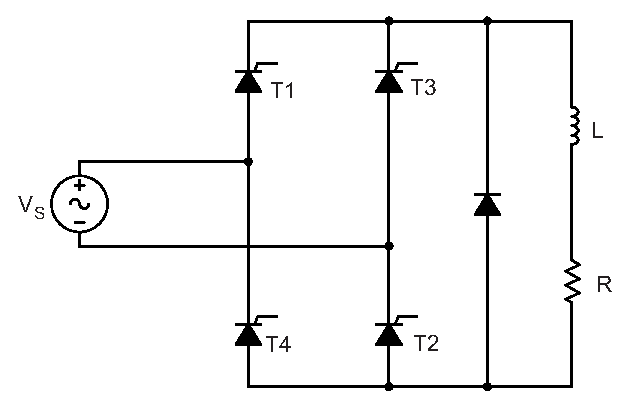
\includegraphics[width=0.6\textwidth]{Caps/Figs/exemplo.eps}
        \fonte{Autoria Própria}
        \label{fig:figura-exemplo1}
    \end{figure}
    
    O código utilizado para inserir a \autoref{fig:figura-exemplo1} está listado no \autoref{qua:figura}.
    
    \begin{quadro}[!htb]
    \centering
    \caption{Código exemplo utilizado para inserir a \autoref{fig:figura-exemplo1} \label{qua:figura}}
    \begin{tabular}{|c|l|}
        \hline
        1 &\verb|\begin{figure}[!htb]|\\
        2 &\verb|\centering|\\
        3 &\verb|\caption{Exemplo de Figura}|\\
        4 &\verb|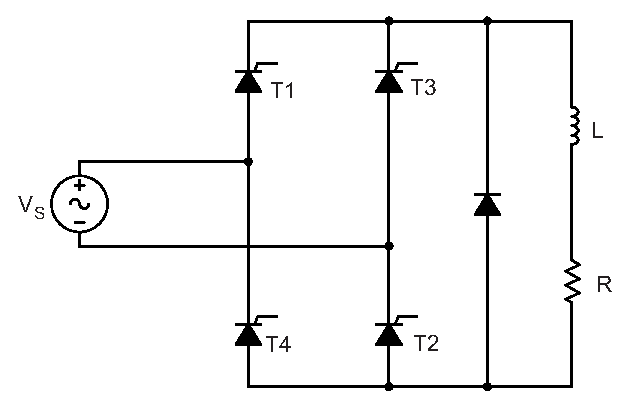
\includegraphics[width=0.6\textwidth]{Caps/Figs/exemplo.eps}|\\
        5 &\verb|\fonte{Autoria Própria}|\\ 
        6 &\verb|\label{fig:figura-exemplo1}|\\ 
        7 &\verb|\end{figure}|\\ 
        \hline
    \end{tabular}
    \fonte{Autoria própria}
    \end{quadro}
    
    Utilize figuras no formato \textit{Encapsulated PostScript} (EPS)\nomenclature[A]{EPS}{\textit{Encapsulated PostScript}}. Caso precise de outro formato, acrescente no preambulo deste modelo o pacote adequado para a sua necessidade.
    
\section{QUADROS E TABELAS}
\label{sec:tabelas}

    Esta seção trata de exemplos de como inserir o \autoref{qua:quadro-exemplo1} e a \autoref{tab:tabela-exemplo1}. Ambos aparecem automaticamente nas suas respectivas listas. Para saber mais informações sobre a construção de tabelas no \LaTeX{} consulte literatura especializada \cite{Mittelbach2004}.

    \begin{quadro}[!htb]
    \centering
    \caption{Exemplo de Quadro \label{qua:quadro-exemplo1}}
    \begin{tabular}{|p{7cm}|p{7cm}|}
        \hline
        \textbf{BD Relacionais} & \textbf{BD Orientados a Objetos} \\
        \hline
        Os dados são passivos, ou seja, certas operações limitadas podem ser automaticamente acionadas quando os dados são usados. Os dados são ativos, ou seja, as solicitações fazem com que os objetos executem seus métodos. & Os processos que usam dados mudam constantemente. \\
        \hline
    \end{tabular}
    \fonte{\citeonline{Barbosa2004}}
    \end{quadro}

    A diferença entre quadro e tabela está no fato que um quadro é formado por linhas horizontais e verticais. Deve ser utilizado quando o conteúdo é majoritariamente não-numérico. O número do quadro e o título vem acima do quadro, e a fonte, deve vir abaixo. Uma tabela é formada apenas por linhas verticais. Deve ser utilizada quando o conteúdo é majoritariamente numérico. O número da tabela e o título vem acima da tabela, e a fonte, deve vir abaixo, tal como no quadro.

    \begin{table}[!htb]
    \centering
    \caption[Resultado dos testes]{Resultado dos testes
    \label{tab:tabela-exemplo1}}
    \begin{tabular}{rrrrr}
        \toprule
            & Valores 1 & Valores 2 & Valores 3 & Valores 4 \\
        \midrule
            Caso 1 & 0,86 & 0,77 & 0,81 & 163 \\
            Caso 2 & 0,19 & 0,74 & 0,25 & 180 \\
            Caso 3 & 1,00 & 1,00 & 1,00 & 170 \\
        \bottomrule
    \end{tabular}
    \fonte{\citeonline{Barbosa2004}}
    \end{table}
    
    Os códigos para inserção do \autoref{qua:quadro-exemplo1} e da \autoref{tab:tabela-exemplo1} estão disponíveis nos Quadros \ref{qua:quaex} e \ref{qua:tabex}.
    
    \begin{quadro}[!htb]
    \centering
    \caption{Código exemplo utilizado para inserir o \autoref{qua:quadro-exemplo1} \label{qua:quaex}}
    \begin{tabular}{|p{0.9\linewidth}|}
    \hline
    \begin{verbatim}
\begin{quadro}[!htb]
\centering
\caption{Exemplo de Quadro \label{qua:quadro-exemplo1}}
    \begin{tabular}{|p{7cm}|p{7cm}|}
    \hline
    \textbf{BD Relacionais} & \textbf{BD Orientados a Objetos} \\
    \hline
    Os dados são passivos, ou seja, certas operações limitadas 
    podem ser automaticamente acionadas quando os dados são 
    usados. Os dados são ativos, ou seja, as solicitações fazem 
    com que os objetos executem seus métodos. & Os processos 
    que usam dados mudam constantemente. \\
    \hline
    \end{tabular}
\fonte{\citeonline{Barbosa2004}}
\end{quadro}
    \end{verbatim}
    \\
    \hline
    \end{tabular}
    \fonte{Autoria própria}
    \end{quadro}
    
    \begin{quadro}[!htb]
    \centering
    \caption{Código exemplo utilizado para inserir a \autoref{tab:tabela-exemplo1} \label{qua:tabex}}
    \begin{tabular}{|p{0.9\linewidth}|}
    \hline
    \begin{verbatim}
\begin{table}[!htb]
\centering
\caption[Resultado dos testes]{Resultado dos testes
\label{tab:tabela-exemplo1}}
    \begin{tabular}{rrrrr}
        \toprule
            & Valores 1 & Valores 2 & Valores 3 & Valores 4 \\
        \midrule
            Caso 1 & 0,86 & 0,77 & 0,81 & 163 \\
            Caso 2 & 0,19 & 0,74 & 0,25 & 180 \\
            Caso 3 & 1,00 & 1,00 & 1,00 & 170 \\
        \bottomrule
    \end{tabular}
\fonte{\citeonline{Barbosa2004}}
\end{table}
    \end{verbatim}
    \\
    \hline
    \end{tabular}
    \fonte{Autoria própria}
    \end{quadro}
    
\section{EQUAÇÕES}
\label{sec:equacoes}

    Esta seção trata de exemplos de como inserir a Eq. (\ref{eq:equacao-exemplo1}) e a Eq. (\ref{eq:equacao-exemplo2}) no corpo do texto \footnote{Deve-se atentar ao fato de a formatação das equações ficar ótima esteticamente.}. Observe que foram utilizadas duas formas distintas para referenciar as equações. Os códigos utilizados estão no \autoref{qua:eqex}.

    \begin{equation}
        X(s) = \int\limits_{t = -\infty}^{\infty} x(t)  \mathrm{e}^{-st}  dt
        \label{eq:equacao-exemplo1}
    \end{equation}

    \begin{equation}
        F(u, v) = \sum_{m = 0}^{M - 1} \sum_{n = 0}^{N - 1} f(m, n) \exp \left[ -j 2 \pi \left( \frac{u m}{M} + \frac{v n}{N} \right) \right]
        \label{eq:equacao-exemplo2}
    \end{equation}
    
    \begin{quadro}[!htb]
    \centering
    \caption{Código exemplo utilizado para inserir as Equações (\ref{eq:equacao-exemplo1}) e (\ref{eq:equacao-exemplo2}) \label{qua:eqex}}
    \begin{tabular}{|p{0.9\linewidth}|}
    \hline
    \begin{verbatim}
\begin{equation}
    X(s) = \int\limits_{t = -\infty}^{\infty} x(t)\text{e}^{-st}dt
    \label{eq:equacao-exemplo1}
\end{equation}

\begin{equation}
    F(u, v) = \sum_{m = 0}^{M - 1} \sum_{n = 0}^{N - 1} f(m, n) 
    \exp \left[ -j 2 \pi \left( \frac{u m}{M} + \frac{v n}{N} 
    \right) \right]
    \label{eq:equacao-exemplo2}
\end{equation}
    \end{verbatim}
    \\
    \hline
    \end{tabular}
    \fonte{Autoria própria}
    \end{quadro}
    
\section{SOBRE AS LISTAS}
\label{sec:apSobreLista}

    Exemplo de duas listas não numeradas aninhadas, utilizando o comando \verb|\itemize|. Observe a indentação, bem como a mudança automática do tipo de "\textit{bullet}"{} nas listas aninhadas.

    \begin{itemize}
        \item item não numerado 1
        \item item não numerado 2
        \begin{itemize}
            \item subitem não numerado 1
            \item subitem não numerado 2
            \item subitem não numerado 3
        \end{itemize}
        \item item não numerado 3
    \end{itemize}

    Exemplo de duas listas numeradas aninhadas, utilizando o comando \verb|\enumerate|. Observe a numeração progressiva e indentação das listas aninhadas.

    \begin{enumerate}
        \item item numerado 1
        \item item numerado 2
        \begin{enumerate}
            \item subitem numerado 1
            \item subitem numerado 2
            \item subitem numerado 3
        \end{enumerate}
        \item item numerado 3
    \end{enumerate}
    
\subsection{CITAÇÕES INDIRETAS}
\label{subsec:citacoesLivres}

    É a transcrição, com suas próprias palavras, das idéias de um autor, mantendo-se o sentido original. A citação indireta é a maneira que o pesquisador tem de ler, compreender e gerar conhecimento a partir do conhecimento de outros autores. Quanto à chamada da referência, ela pode ser feita de duas maneiras distintas, conforme o nome do(s) autor(es) façam parte do seu texto ou não. Exemplo de chamada fazendo parte do texto:
    
    \vspace{1cm}
    
    Enquanto \citeonline{Maturana2003} defendem uma epistemologia baseada na biologia. Para os autores, é necessário rever \ldots
    
    \vspace{1cm}

    A chamada de referência foi feita com o comando \verb|\citeonline{chave}|, que produzirá a formatação correta.

    A segunda forma de fazer uma chamada de referência deve ser utilizada quando se quer evitar uma interrupção na sequência do texto, o que poderia, eventualmente, prejudicar a leitura. Assim, a citação é feita e imediatamente após a obra referenciada deve ser colocada entre parênteses. Porém, neste caso específico, o nome do autor deve vir em caixa alta, seguido do ano da publicação. Exemplo de chamada não fazendo parte do texto:
    
    \vspace{1cm}
    
    Há defensores da epistemologia baseada na biologia que argumentam em favor da necessidade de \ldots \cite{Maturana2003}.
    
    \vspace{1cm}
    
    Nesse caso a chamada de referência deve ser feita com o comando \verb|\cite{chave}|, que produzirá a formatação correta.
    
\subsection{CITAÇÕES DIRETAS}
\label{subsec:citacoesLiterais}

    É a transcrição ou cópia de um parágrafo, de uma frase, de parte dela ou de uma expressão, usando exatamente as mesmas palavras adotadas pelo autor do trabalho consultado.

    Quanto à chamada da referência, ela pode ser feita de qualquer das duas maneiras já mencionadas nas citações indiretas, conforme o nome do(s) autor(es) façam parte do texto ou não. Há duas maneiras distintas de se fazer uma citação direta, conforme o trecho citado seja longo ou curto.

    Quando o trecho citado é longo (4 ou mais linhas) deve-se usar um parágrafo específico para a citação, na forma de um texto recuado (4 cm da margem esquerda), com tamanho de letra menor e espaçamento entrelinhas simples. Exemplo de citação longa:
    
    \vspace{1cm}
    
    \begin{citacao}
        Desse modo, opera-se uma ruptura decisiva entre a reflexividade filosófica, isto é a possibilidade do sujeito de pensar e de refletir, e a objetividade científica. Encontramo-nos num ponto em que o conhecimento científico está sem consciência. Sem consciência moral, sem consciência reflexiva e também subjetiva. Cada vez mais o desenvolvimento extraordinário do conhecimento científico vai tornar menos praticável a própria possibilidade de reflexão do sujeito sobre a sua pesquisa \cite[p.~28]{Silva2000}.
    \end{citacao}

    Para fazer a citação longa deve-se utilizar os seguintes comandos:
    \begin{verbatim}
\begin{citacao}
<texto da citacao>
\end{citacao}
    \end{verbatim}

    No exemplo, para a chamada da referência o comando \verb|\cite[p.~28]{Silva2000}| foi utilizado, visto que os nomes dos autores não são parte do trecho citado. É necessário também indicar o número da página da obra citada que contém o trecho citado.

    Quando o trecho citado é curto (3 ou menos linhas) ele deve inserido diretamente no texto entre aspas. Exemplos de citação curta:
    
    \vspace{1cm}
    
    A epistemologia parte do princípio de que "assumo que não posso fazer referência a entidades independentes de mim para construir meu explicar" \cite[p.~35]{Maturana2003}.
    
    \vspace{1cm}
    
    A epistemologia baseada na biologia de \citeonline[p.~35]{Maturana2003} parte do princípio de que "assumo que não posso fazer referência a entidades independentes de mim para construir meu explicar".
    
\section{SOBRE AS REFERÊNCIAS BIBLIOGRÁFICAS}
\label{sec:apSobreRefer}

    A bibliografia é feita no padrão \textsc{Bib}\TeX{}. As referências são colocadas em um arquivo separado. Neste template as referências são armazenadas no arquivo 

\begin{center}
``references.bib''.
\end{center}

Existem diversas categorias documentos e materiais componentes da bibliografia. A classe abn\TeX{} define as seguintes categorias (entradas):

\begin{verbatim}
@book
@inbook
@article
@phdthesis
@mastersthesis
@monography
@techreport
@manual
@proceedings
@inproceedings
@journalpart
@booklet
@patent
@unpublished
@misc
\end{verbatim}

Cada categoria (entrada) é formatada pelo pacote \citeonline{abnTeX22014d} de uma forma específica. Algumas entradas foram introduzidas especificamente para atender à norma \citeonline{NBR6023:2002}, são elas: \verb|@monography|, \verb|@journalpart|,\verb|@patent|. As demais entradas são padrão \textsc{Bib}\TeX{}. Para maiores detalhes, refira-se a \citeonline{abnTeX22014d}, \citeonline{abnTeX22014b}, \citeonline{abnTeX22014c}.

% NOTAS DE RODAPÉ--------------------------------------------------------------------------
\section{NOTAS DE RODAPÉ}
\label{sec:notasRodape}

As notas de rodapé pode ser classificadas em duas categorias: notas explicativas\footnote{É o tipo mais comum de notas que destacam, explicam e/ou complementam o que foi dito no corpo do texto, como esta nota de rodapé, por exemplo.} e notas de referências. A notas de referências, como o próprio nome ja indica, são utilizadas para colocar referências e/ou chamadas de referências sob certas condições.




    
    % O TCC 1 deve conter:
    %   1 - Introdução
    %   2 - Objetivos
    %   3 - Justificativa
    %   4 - Referencial teórico
    %   5 - Materiais e métodos
    %   6 - Resultados esperados
    %   7 - Cronograma
    
    
    % Bibliografia
    \bibliography{references}
    
    \postextual
    
    % Apêndices:
    \apendices
    %\chapter{Título do Apêndice}
\label{apen:apen1}

\lipsum
    
    % Anexos:
    \anexos
    %\chapter{Título do Anexo}
\label{anex:anex1}

\lipsum
    
\end{document}
